
\documentclass[12pt]{article}

\title{A spatial stochastic discount factor estimator for private equity funds}

\author{
	Christian Tausch  \\
	AssetMetrix GmbH  \\
	Theresienh\"{o}he 13, D-80339 Munich \\
	christian.tausch@quant-unit.com \\
	% \and 
	}

\date{\today}



% Packages
\usepackage{amssymb}
\usepackage{amsmath}
\usepackage{natbib}
\usepackage{graphics}
% use smaller margins
\usepackage[margin=1.0in]{geometry} % 1.25in
% use double spacing
\usepackage{setspace}
\usepackage{amsthm}
\usepackage{url}
\usepackage[outdir=eps]{epstopdf}


\newtheorem{prop}{Proposition}
\newtheorem{assume}{Assumption}

\begin{document}

\maketitle


\section*{Keywords}
Stochastic discount factor, Semiparametric, M-estimation, Spatial inference, Private equity fund, Fund level data


\section*{Acknowledgements}
I thank Hsin-Chih Ma, Stefan Mittnik, Daniel Schalk, Nicolas D\"{u}tsch and all participants of the LMU econometrics research seminar SS 2019 for helpful discussions and support.


\section*{Declaration of interest}
The author reports no conflict of interest. 
The author alone is responsible for the content and writing of the paper.


\newpage
\doublespacing

\begin{center} 
\section*{A spatial stochastic discount factor estimator for private equity funds}
\end{center}



\begin{abstract}
This paper proposes an improved stochastic discount factor estimation methodology suited for fund-level cash flows of private equity funds.
The asymptotic inference framework for this semiparametric least-mean-distance estimator draws on a spatial notion, i.e., the idea that the economic distance between distinct private equity funds can be measured.
The empirical and Monte Carlo simulation results reveal high estimator variance for typical data sizes.
Thus, we conjecture that naive semiparametric M-estimators like ours shall be exclusively used for single-factor models until considerably more vintage year information for private equity funds is available.
\end{abstract}


%% main text
\section{Introduction}

Do investments in Private Equity (PE) funds offer abnormal returns to fund investors when risk-adjusted for public market factors?
Currently, a popular approach to answer this question is to evaluate private equity fund cash flows by Stochastic Discount Factor (SDF) models that draw on public market return covariates.
The basic idea for SDF model estimation is that the sum of all discounted fund net cash flows is expected to be zero when the true SDF is applied.
Unfortunately, there is no conclusion about the best methodology to estimate these SDF models, as a variety of proposals coexists in the academic private equity fund literature \citep{DLP12,B14,KN16,ACGP18,GSW19}.

This paper aims to revise and enhance existing semiparametric approaches.
Especially our conclusions from the insightful \cite{DLP12} and \cite{KN16} articles lead us to suggest an improved Least-Mean-Distance (LMD) estimator for SDF models.
It can be applied to fund-level cash flow data of private equity funds.
On the one hand, we provide asymptotic inference formulations that rely on the concept of spatial (near-epoch) dependence between funds following the pioneering idea in \cite{KN16}.
In this context, it is paramount to quantify the economic distance between funds by a measure like absolute vintage year difference or cash flow overlap\footnote{However, this economic inter-fund \emph{distance} refers \textbf{not} to the term Least-Mean-\emph{Distance} estimator.}.
On the other hand, our LMD estimator arguably generalizes the \cite{DLP12} methodology, where we provide the asymptotic inference framework that was missing in the original paper.
Additionally, we propose a simple solution to the 'exploding alpha' issue briefly mentioned in their paper.
Our Monte Carlo results suggest that the same modification dramatically reduces the inherent small-sample bias associated with the original \cite{DLP12} estimator.

In the empirical application of our new estimator, we test simple linear and exponentially affine SDF models that can draw on the five return factors associated with the $q^5$ investment factor model recently proposed by \cite{HXZ20}.
Based on a Spatial Heteroskedasticity and Autocorrelation Consistent (SHAC) covariance matrix estimator, we calculate asymptotic standard errors for the model coefficients.
Moreover, we assess the small-sample variance of coefficient estimates and the out-of-sample performance of the different SDF models by $hv$-block cross-validation, which accounts for the inter-vintage-year dependence of private equity funds \citep{R00}.
We test one- and two-factor models for the following private equity fund types: Private Equity, Venture Capital, Private Debt, Real Estate, Natural Resources, and Infrastructure.
All two-factor model results are rather devastating; not more than the single-market-factor model results seem reasonable given the high estimator variance.

The paper is structured as follows. 
Section \ref{sec:Methodology} introduces our semiparametric LMD estimator and its corresponding asymptotic inference framework.
Section \ref{sec:empirical_application} applies the method to estimate $q^5$-investment-factor SDFs for various private equity fund types using simulated and real-world cash flows.
Section \ref{sec:conclusion} concludes.


\section{Methodology}
\label{sec:Methodology}

\subsection{Least-Mean-Distance estimator}
\label{sec:fundwise_lmd_estimator}

Our general SDF setting is similar to that of \cite{DLP12} and \cite{KN16}; the subtle differences are discussed in section \ref{sec:comparison_to_similar_estimators}.

Let fund $i=1,2,\dots,n$ be characterized by its net cash flows ${CF}_{t,i}$ (i.e., distributions minus contributions) and its net asset values ${NAV}_{t,i}$ with discrete time index $t=1,2,\dots,T$.
The data generating processes (DGPs) for $CF$ and $NAV$ are left unspecified.
For a non-liquidated fund we treat the most recent NAV as final distribution cash flow.
The stochastic discount factor $\Psi_{\tau,t}$ can be used to calculate the (realized) time-$\tau$ price $P_{\tau,t,i}$ of a \textbf{single} time-$t$ cash flow of any given PE fund $i$
\begin{equation}
\label{eq:price}
P_{\tau,t,i} = \Psi_{\tau,t} \cdot CF_{t,i}
\qquad \forall \quad \tau,t,i
\end{equation}
As SDFs are commonly parameterized by a vector $\theta \in \mathbb{R}^{p}$, i.e., $\Psi_{t,\tau} \equiv \Psi_{t,\tau} (\theta)$, our goal is to find an estimation method for the optimal $\theta$.
For each fund $i$ and all points $\tau$ within a common fund lifetime, the pricing error $\epsilon_{\tau,i}$ of \textbf{all} fund cash flows is calculated as net present value
\begin{equation}
\label{eq:pricing_error}
\epsilon_{\tau,i} = \sum_{t=1}^T P_{\tau,t,i} 
\qquad \forall \quad \tau,i
\end{equation}
We define the $w_i$-weighted and $\mathcal{T}_i$-averaged fund pricing error as
\begin{equation}
\label{eq:average_pricing_error}
\bar{\epsilon}_{i} =
w_{i} \cdot
\frac{1}{ \mathrm{card}(\mathcal{T}_{i}) }
\sum_{\tau \in \mathcal{T}_{i}}
\epsilon_{\tau,i}
\qquad \forall \quad i
\end{equation}
where $\mathcal{T}_i$ gives the set of (relevant) present value times $\tau$ for fund $i$ (cf. figure \ref{fig:npvs}).
A present value date $\tau \in \mathcal{T}_{i}$ is a discretionary time point where all fund cash flows are discounted to.
The cardinality $\mathrm{card}(\mathcal{T}_{i})$ gives the number of present value dates used for the $i$th fund.
The smallest possible set $\mathcal{T}_i$ contains just a fund's starting date; in this case, $\mathrm{card}(\mathcal{T}_{i})$ consequently is one.
The largest set contains all time periods bigger than the fund's starting date until now.
The optimal set size of $\mathcal{T}$ is studied by Monte Carlo simulations in subsection \ref{sec:simulation_study}.
There we show that controlling for the optimal size of $\mathcal{T}$ decreases the small-sample bias and variance of the original \cite{DLP12} estimator that just discounts all cash flows to the fund inception date.
Additionally, each fund $i$ is characterized by its vintage year which can be expressed by $v_{i}=\min(\mathcal{T}_i) \in 1,2,\dots,V$, where $V$ denotes the maximum vintage year used in a given data set.
Finally, the scalar weighting factor $w_i$ can be (i) one divided by the fund's invested capital for equal weighting of funds, (ii) one divided by the vintage year sum of invested capital for vintage year weighting, (iii) the scalar one for fund-size weighting, or (iv) some macroeconomic deflator.

To find $\theta$, our LMD estimator minimizes the average loss of $\bar{\epsilon}$
\begin{equation}
\label{eq:estimator}
\hat{\theta} = 
\mathrm{arg \ min}_{\theta \in \Theta}
\enspace
S_n(\theta)
\quad
\mathrm{with}
\quad
S_n(\theta) = 
\frac{1}{n}
\sum_{i=1}^n
L \left( \bar{\epsilon}_{i} \right) 
\end{equation}
where $L$ denotes a loss function, e.g., $L(x)=(x-0)^2$.
Throughout the paper, the weighted average fund pricing error $\bar{\epsilon} \equiv \bar{\epsilon}(\theta)$ is regarded as nonlinear random function of the SDF parameter $\theta$.

\begin{figure}[ht]
	\centering
	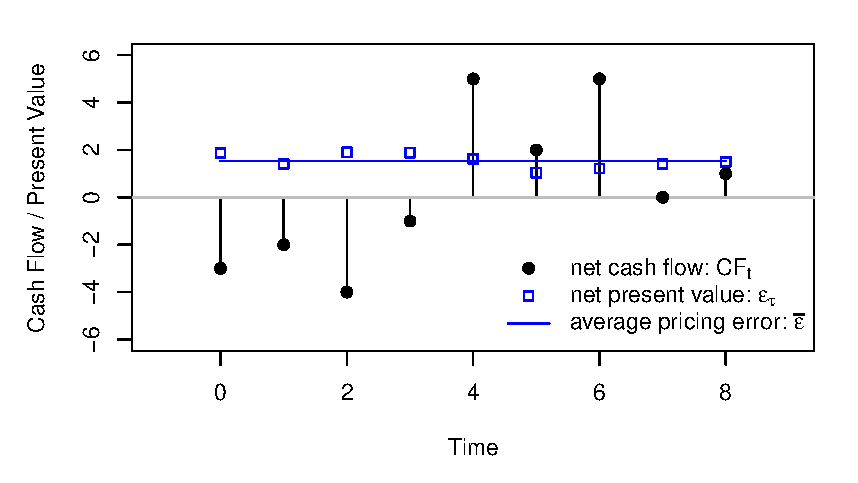
\includegraphics{eps/npvs.eps}
	\caption{
		How to calculate and interpret the average pricing error?
		The time index $t$ is relevant for the net cash flows (black dots).
		The time index $\tau$ is used for the net present values of this net cash flow stream (blue boxes).
		The weighted average of these net present values gives the average pricing error $\bar{\epsilon}$ as defined in equation \ref{eq:average_pricing_error} (solid blue line).
	}
	\label{fig:npvs}
\end{figure}

\subsection{Cross-sectional unit: Individual fund vs. portfolio of funds}
\label{sec:cross_sectional_unit}

According to the classical value-additivity assumption in \cite{HR87} SDF models invariably shall hold for all pooled or unpooled assets.
So, in theory, it is not important if the test assets for our SDF are portfolio or individual fund cash flows.
Practically it makes a difference and there are arguments both for and against portfolio formation.

In the risk premium literature, portfolio formation mainly helps to attenuate the errors-in-variables bias connected to two-pass asset pricing methods \citep{JNPR19,PRS19}.
As this is no issue in our case, we could use individual funds.
\cite{C11} argues that portfolio sorting (seen as an auxiliary nonparametric regression that imposes linearity on the relationship between returns and characteristics) shall be replaced by multivariate panel models due to the curse of dimensionality.
Following the same nonparametric regression viewpoint, \cite{CCF19} derive a nonparametric framework where the optimal number of portfolios sorts acts as a data-dependent tuning parameter that grows with sample size.
Generally, the larger the portfolios, the easier any given SDF can price their cash flows since fewer test assets remain.

In the case of private equity funds, the pooling of fund cash flows helps to counter GP financial engineering\footnote{GPs may use bridge credit facilities below the hurdle rate to boost the fund's internal rate of return. This increases the probability of observing funds with only positive or only negative cash flows. Yet, we want to avoid (the possibility of) cross-sectional units that exhibit just cash flows with the same algebraic sign. Realistic SDFs never can price these cash flow streams.}, which might both change and mask the true risk profile of observed LP cash flows.
Especially for private equity funds, portfolio formation based on vintage year is compelling due to its time-series-like indexing as done by \cite{DLP12}.
This procedure also offers substantial computational benefits as it drastically decreases the number of cross-sectional units.
Further, as stated in \cite{ALS20}, portfolio formation allows more precise factor loading estimates  due to decreasing idiosyncratic risk, but at the expense of sacrificing cross-sectional information.
Finally, small (or fixed) $T$ and large $N$ set-ups may face finite sample problems \citep{RRZ20}.

\begin{assume}
	\label{as:portfolio}
	For each vintage year, we pool fund cash flows to form $n_v$ portfolios that serve as cross-sectional units.
	The two boundary cases are (i) single fund portfolios and (ii) just one portfolio per vintage year. 
\end{assume}
Without loss of generality, we refer to our cross-sectional units as funds, although this is just a special case of a size-$n_v$-portfolio.
In the simulation study in subsection \ref{sec:simulation_study}, we compare both boundary cases (i) individual funds and (ii) vintage year portfolios.


\subsection{Asymptotic framework}
\label{sec:asymptotic_framework}

To allow for multiple funds from the same vintage year in assumption \ref{as:portfolio}, we employ an auxiliary 'spatial' notion as originally proposed by \cite{KN16}.
The spatial viewpoint is just a technical means to switch from time-series-like to more panel-data-like indexing.
Unlike typical panel data, we do not follow multiple subjects over time, but for each point in time, we exclusively observe multiple new cross-sectional units (i.e., funds from that vintage year).
This unusual two-dimensional indexing causes problems in the PE literature as it neatly fits neither in the (i) time-series, (ii) cross-sectional, nor (iii) panel data literature.

However, in this section, we mainly follow the time-series asymptotic framework of \cite{PP97} since our 'spatial' distance measure is time and adaption to our case is thus straightforward.
If we observe just one fund per vintage year (or, equivalently, form vintage year portfolios), we can easily see that the framework of \cite{PP97} with time-series indexing can be directly applied (without any major modification).


\subsubsection{Vintage year asymptotics}
We assume that the 'spatial' (i.e., economic) distance between cross-sectional units, i.e., private equity funds/portfolios, can be measured quantitatively\footnote{Generally, the economic distance measure could include multiple dimensions, e.g., temporal, geographic, and industry sector proximity.}.
Here our asymptotic theory lets the number of funds go to infinity $n \to \infty$.
However, to expose our SDF to enough distinct covariate realizations (economic conditions), identification of model parameters requires a sufficient number of funds from different vintage years in the fund-level data set used for model estimation as emphasized by \cite{DLP12} and \cite{KN16}.
\begin{assume}
	\label{as:vya}
	(i) The number of vintage years $V \to \infty$ as $n \to \infty$.
	(ii) The number of funds per vintage year is bounded by some positive constant.
	(iii) The maximal fund lifetime is also bounded by a positive constant.
	(iv) The economic distance between fund $i$ and $j$ is measured by the vintage year difference $d_{i,j}=v_i - v_j$.
\end{assume}
In terms of the spatial estimation literature, this assumption postulates increasing domain asymptotics and rules out so-called infill asymptotics. Infill asymptotics corresponds to the assumption of \cite{DLP12} that the number of funds per vintage tends to infinity.


\subsubsection{Law of large numbers}
The global moment condition underlying our estimation approach is that the expected value of $\bar{\epsilon}$ shall be zero if we use the optimal SDF parameter $\theta_0$. 
This technically means, instead of applying a time-series law of large numbers, we rely on a spatial (cross-sectional) law of large numbers, but acknowledge the statistical dependence of  pricing errors from adjacent vintage years.

\begin{assume}
	\label{as:lln}
	The (i) time-trend and (ii) dependence structure of $\bar{\epsilon}$ shall allow
	\[
	n^{-1} \sum_{i=1}^n \overline{\epsilon}_i \overset{a.s.}\to E[\bar{\epsilon}]
	\quad {as} \quad V,n \to \infty
	\]
	Specifically, we assume the process $\overline{\epsilon}$ to be is spatial near-epoch dependent with respect to fund vintage years \citep{JP12}, i.e., two funds with distance $d_{i,j}>D$ are assumed to be independent.
\end{assume}
To satisfy the time trend part (i) of this law of large number assumption, the weighting factor $w$, introduced in equation \ref{eq:average_pricing_error}, can be used to make $\bar{\epsilon}$ stationary.
Spatial near-epoch dependence with respect to fund vintage years formalizes the simple idea that two fund pricing errors $\bar{\epsilon}$ with a small absolute vintage year difference are supposed to be dependent sine they are exposed to the same macroeconomic conditions.
In contrast, two funds with a large absolute vintage year difference can be assumed independent.

\subsubsection{Consistency}
The estimator $\hat{\theta}$ shall converge in probability to the true parameter value $\theta_0$ as the number of distinct vintage years in our data set goes to infinity.
Multiple funds for a specific vintage year are not necessarily required but provide additional information that we want to exploit if available.

\begin{assume}
\label{as:consistency}
 Consistency of $\hat{\theta}$ requires $\hat{\theta} \overset{p}{\to} \theta_0$ as $V,n \to \infty$.
 Thus $E[\bar{\epsilon}]=0$ if and only if $\theta=\theta_0$.
 The parameter space is compact $\theta \in \Theta$.
\end{assume}
Compactness of $\Theta$ can be assured by lower and upper bounds for all parameters that can be justified by economic reasoning. In our case, e.g., a market beta factor of ten seems implausible for PE funds because of the implied risk and return expectations.

\subsubsection{Central limit theorem}
To assess the large-sample significance of our parameter estimates (in the following subsection \ref{sec:asymptotic_inference}), we want to describe the asymptotic distribution of the parameter vector as a normal distribution.

\begin{assume}
	\label{as:clt}
	(i) $\sqrt{n}(\hat{\theta} - \theta_0) \overset{d}{\to} \mathcal{N}(0,\mathbf{\Sigma})$ as $V,n \to \infty$ with covariance matrix $\mathbf{\Sigma}$.
	
	(ii) The covariance matrix $\mathbf{\Sigma}$ can be characterized by \citet[Theorem 11.2.b, Theorem H.1]{PP97}.
\end{assume}

The formal proof of assumption \ref{as:clt} may be derived in analogy to the GMM case in \cite[Theorem 4]{JP12} that shows that the general structure of the \cite{PP97} framework also applies to the spatial near-epoch dependent case.



\subsection{Large sample inference}
\label{sec:asymptotic_inference}

In the time-series near-epoch-dependent LMD literature, the covariance matrix $\mathbf{\Sigma}$ can be characterized according to \citet[Theorem 11.2.b, Theorem H.1]{PP97}:
\[
\mathbf{\Sigma} = C^{-1} \Lambda (C^{-1})^\top
\]
with expected Hessian matrix converging to $C$ as $V,n \to \infty$
\[
E 
\left(
\nabla_{\theta \theta} S_n
\right)
\to C
\]
and the expected covariance matrix of gradients converging to $\Lambda$ as $V,n \to \infty$
\[
n E 
\left[
\nabla_{\theta} S_n
(\nabla_{\theta} S_n)^\top
\right]
\to \Lambda
\]
Here, the gradient vector $\nabla_{\theta} S_n$ is denoted as column vector.
We define the corresponding finite sample estimators analogously to \citet[Chapters 12, 13.1]{PP97}, and numerically approximate the first and second partial derivatives by finite differences ($\delta \to 0$): 
\[
f_{x}(x,y) \approx \frac{f(x+\delta,y) - f(x-\delta,y)}{2\delta}
\]
\[
f_{xx}(x,y) \approx \frac{f(x+\delta,y) + f(x-\delta,y) - 2  f(x,y)}{\delta^2}
\]
\[
f_{xy}(x,y) \approx \frac{f(x+\delta,y+\delta) + f(x-\delta,y-\delta) -  f(x+\delta,y-\delta) - f(x-\delta,y+\delta)}{4\delta^2}
\]
$\hat{C}$ is relatively straightforward
\[
\hat{C} = \frac{1}{n} \sum_{i=1}^n \nabla_{\theta \theta} L \left( \epsilon_i \right)
\]
Due to the spatial near-epoch dependence, the involved and computationally expensive part is to consistently estimate $\hat{\Lambda}$ by a Spatial Heteroskedasticity and Autocorrelation Consistent (SHAC) covariance matrix estimator \cite[equation 2]{KS11}
\begin{equation}
\label{eq:hac}
\hat{\Lambda} = \frac{1}{n} \sum_{i=1}^n \sum_{j=1}^n
k_{i,j}
\left[
\nabla_{\theta} L \left( \epsilon_i \right)
\left(
\nabla_{\theta} L \left( \epsilon_j \right)
\right)^\top
\right]
\end{equation}
We define the kernel weight $k$ as
\[
k_{i,j} \equiv K \left( \frac{d_{i,j}}{b_n} \right)
\]
with kernel function $K: \mathbb{R} \to [0,1]$ satisfies $K(0)=1$, $K(x)=K(-x)$, $\int_{-\infty}^{\infty} K^2(x) dx < \infty$, and $K(\cdot)$ continuous at zero and at all but a finite number of other points.
A common choice is the Bartlett kernel $K_{BT}(x)= \max(0, 1-|x|)$; see equation 2.7 in \cite{A91} for other popular kernel choices.
This means absolute vintage year differences larger than the bandwidth (or truncation) parameter $b_n=D$ are considered independent and are thus excluded from the $\hat{\Lambda}$ estimation formula.

In large samples, the vector of parameter standard errors can thus be estimated by
\[
\mathrm{SE}(\hat{\theta}) = 
\sqrt{
	\mathrm{diag} \left[
	n^{-\frac{1}{2}}
	\hat{C}^{-1} \hat{\Lambda} (\hat{C}^{-1})^\top
	(n^{-\frac{1}{2}})^\top
	\right] 
}
=
\sqrt{
	\mathrm{diag} \left[
	\hat{C}^{-1} \hat{\Lambda} (\hat{C}^{-1})^\top
	\right] 
	\cdot \frac{1}{n}
}
\]
\iffalse
The Wald test statistic for linear hypotheses $H_0: R \theta = r$ and $H_1: R \theta \neq r$ is constructed as
\[
W = 
(R \hat{\theta} - r)^\top
\left[
R
\frac{\hat{C}^{-1} \hat{\Delta} (\hat{C}^{-1})^\top}{n}
R^\top
\right]^{-1}
(R \hat{\theta} - r)
\stackrel{H_0}{\sim}
\chi_q^2
\]
where $\hat{\theta}$ is the $p \times 1$ parameter vector, $R$ is a $q \times p$ matrix, and $r$ is a $q \times 1$ vector.
Usually, we select $R$ as $p \times p$ identity matrix, and $r$ as $p \times 1$ vector (e.g., of zeros).
Under the null hypothesis, $W$ is chi-squared distributed with $q$ degrees of freedom. As large values of $W$ indicate the rejection of $H_0$, the corresponding p-value is calculated as $1 - F_{\chi_q^2}(W)$ where $F_{\chi_q^2}$ is the cumulative distribution function of a chi-squared random variable with $q$ degrees of freedom.
\fi
However, given the limited amount of available private equity data (typically the oldest vintages start in the 1980s), asymptotic characterizations of $\mathbf{\Sigma}$ and $\mathrm{SE}(\hat{\theta})$ are of limited importance. 
In empirical applications, the small sample behavior of an estimation method for private equity data is more relevant than its asymptotic theory.
Moreover, the standard asymptotic distribution associated with an estimator is generally not valid for post-model-selection inference, i.e., if a model selection procedure is applied to find the best model from a collection of competitors \citep{LP05}.


\subsection{Comparison to similar estimators}
\label{sec:comparison_to_similar_estimators}

Our Least-Mean-Distance (LMD) estimator developed in section \ref{sec:fundwise_lmd_estimator} belongs to the class of semiparametric nonlinear M-estimators as defined in \cite{PP97}.
%The estimator exhibits a cross-sectional nature since $S_n(\theta)$ in equation \ref{eq:estimator} takes the sample average with respect to funds rather than with respect to a vintage-year-based time-series.
We intentionally opt against the most prominent semiparametric nonlinear M-estimator framework, i.e., classical time-series Generalized Method of Moments (GMM) \citep{H82,H12}.
A classical GMM approach requires the construction of stationary, ergodic time-series of moment conditions that are used to empirically estimate the expected value of pricing errors in equation \ref{eq:pricing_error}.
The stationarity requirement of classical time-series GMM limits (i) more elaborate weighting-schemes for $w$, like fund-size weighting, and (ii) the usage of fund cash flows from non-realized vintages.

\subsubsection{\cite{DLP12}}

The \cite{DLP12} approach is most closely related to our methodology.
However, they regard vintage year portfolios as their cross-sectional units; we can also use individual funds.
The \cite{DLP12} asymptotic theory assumes the number of funds (or deals) per vintage year portfolio to go to infinity.
Our asymptotic theory lets both (i) the number of vintage years and (ii) the number of funds go to infinity, but bounds the number of funds per vintage year.
Further, \cite{DLP12} discount all fund cash flows just to the first cash flow date (like in a classical net present value calculation).
In contrast, we additionally average over all dates within $\mathcal{T}_{i}$ to alleviate the exploding alpha issue briefly mentioned in their paper (and more thoroughly so in an earlier working paper version).
Although \cite{DLP12} describe their estimator as a one-step GMM approach, we consider it a special case of our LMD estimator.
Specifically, equation \ref{eq:estimator} from our paper is a generalization of equation 3 from their paper.
Consequently, if someone accepts the assumptions from subsection \ref{sec:asymptotic_framework}, our large sample inference framework from subsection \ref{sec:asymptotic_inference} applies to their case without any significant modification.
Finally, \cite{DLP12} apply simple cross-sectional bootstrapping to obtain standard errors; in contrast, in subsection \ref{sec:model_selection} we use a cross-validation technique that is adapted to the near-epoch dependence of the PE fund data.

\subsubsection{\cite{KN16}}

\cite{KN16}, first of all, realized the usefulness of employing an auxiliary spatial framework to establish asymptotic inference results for a fund-level panel dataset of private equity funds.
They measure the economic distance between two private equity funds (by the degree of cash flow overlap) to account for the cross-sectional dependence between funds.
Concretely, their asymptotic inference framework draws on the spatial HAC estimator of \cite{C99}; our spatial HAC framework uses \cite{PP97,KS11,JP12}.
However, they ultimately utilize a classical GMM estimator, thus a time-series law of large numbers.
Specifically, we obtain the estimator of \cite[equation 18]{KN16} in our framework if we replace $S_n(\theta)$ in equation \ref{eq:estimator} by equation \ref{eq:kn16_estimator}.
\begin{equation}
\label{eq:kn16_estimator}
	S_n(\theta) = 
	L \left( 
	\frac{1}{n}
	\sum_{i=1}^n
	\bar{\epsilon}_{i} 
	\right)
	\quad
	\mathrm{with}
	\quad
	L(x)=x^2
\end{equation}
Time-series GMM estimators inherently bear the risk of under-identification, if the corresponding time-series is constructed by pooling all fund cash flows from a given fund type.
Exactly this happens in equation \ref{eq:kn16_estimator} where we consequentially obtain a GMM estimator with just one moment condition.
To counter under-identification, additional characteristic-based fund portfolios could be formed to increase the number of moment conditions per fund type; also, random portfolios combined with bootstrapping make sense.
Yet, \cite{KN16} take another approach and introduce the concept of Generalized Public Market Equivalent (GPME), which elegantly avoids the under-identification issue.
Firstly, a public market SDF model is estimated by pricing public trading strategies that shall replicate PE funds instead of directly pricing the observed PE fund cash flows.
Only in a second step, these public market SDF models are applied to evaluate private equity fund cash flows.

Given these differences, our approach may not be perceived as straightforward generalization of the \cite{KN16} framework.
In contrast, our LMD estimator generalizes the \cite{DLP12} method. 
Table \ref{tab:comparison} summarizes the most prominent distinctions between the three approaches.

\begin{table}[ht]
	\centering
	\resizebox{\textwidth}{!}{%
	\begin{tabular}{llll}
		 & \cite{DLP12} & \cite{KN16} & Our approach \\ 
		\hline
		\hline
		M-estimator & Least-Mean- & Generalized Method & Least-Mean-  \\
		& Distance & of Moments & Distance \\
		\hline
		Pricing error averaging & No & No & Yes \\
		\hline
		Cash flows priced & PE cash flows & public cash flows & PE cash flows \\
		\hline
		Asymptotics & cross-sectional & time-series & spatial \\
		 & \#funds $\to \infty$ & \#vintages $\to \infty$ & \# of both $\to \infty$ \\
		\hline
		Inference & bootstrap & spatial HAC & cross-validation \\
		& & & \& spatial HAC \\
		\hline
		Cross-sectional unit & vintage year portfolio & single fund & testing both \\
		\hline
		SDF & simple linear & exponentially affine & testing both \\
		\hline
		\hline
	\end{tabular}
	}
	\caption{Comparison to similar estimation frameworks.} 
	\label{tab:comparison}
\end{table}



\section{Empirical application}
\label{sec:empirical_application}

\subsection{Data}

We use the Preqin cash flow data set as of 26th February 2020.
We pool all regions and analyze the following fund types (using the Preqin asset class classification):
PE ("Private Equity"; 2248 distinct funds in data set; 36 vintage years),
VC ("Venture Capital"; 871; 36),
RE ("Real Estate"; 742; 27),
PD ("Private Debt"; 441; 31),
INF ("Infrastructure", 144; 17), 
NR ("Natural Resources", 138; 26).
For these fund types, we extract all (i) equal-weighted and (ii) fund-size-weighted cash flow series.
For non-liquidated funds, we treat the latest net asset value as final cash flow.
We explicitly refrain from excluding the most recent vintage years.
Thus, the minimum vintage year is 1983 (just for PE) and the maximum is 2019.

The public market factors that enter our SDF draw on the US data set of the recently popularized $q^5$ investment factor model sourced from \url{http://global-q.org/factors.html} \citep{HXZ15,HXZ20}. 
Their five-factor model includes the market excess return (MKT), a size factor (ME), an investment factor (IA), a return on equity factor (ROE), and an expected growth factor (EG).


\subsection{Model and estimator specifications}
\label{sec:model_selection}
We test a simple linear SDF model as in \cite{DLP12}
\begin{equation}
\label{eq:linear_sdf}
\Psi_{\tau,t}^{\mathrm{SL}} (\theta) = 
\prod_{h=1}^{t}\ \left(1 + \alpha + r_{h} + \sum_j\ \beta_j\ F_{j,h} \right)^{-1}
\prod_{h=1}^{\tau}\ \left(1 + \alpha + r_{h} + \sum_j\ \beta_j \ F_{j,h} \right)
\end{equation}
and an exponential affine SDF model adapted from \cite{KN16}
\begin{equation}
\label{eq:expaff_SDF}
\Psi_{\tau,t}^{\mathrm{EA}} (\theta) = 
\exp
\left[
-
\sum_{h=\tau}^{t} \left( \alpha + \log (1 + r_h) + \sum_{j \in J} \beta_{j} \cdot \log (1 + F_{j,h}) \right)
\right]
\end{equation}
with (arithmetic) risk-free return $r$, (arithmetic) zero-net-investment portfolio returns $F_j$, and parameter vector $\theta=(\alpha,\beta)$.
To avoid overfitting, we just test six simple SDF models that contain \{MKT\} alone or \{MKT\} plus \{ME or IA or ROE or EG or Alpha\}.
In equation \ref{eq:estimator}, we use the quadratic loss function $L(x)=x^2$.

To assess the parameter significance, we compute the asymptotic standard errors as outlined in subsection \ref{sec:asymptotic_inference}.
For the Bartlett kernel's bandwidth $b_n=D$ we select 12 years, i.e., funds with absolute vintage year differences larger than 12 years are assumed to be independent.

Additionally, we want to test the finite - or more honestly small - sample parameter significance and the out-of-sample performance of our SDF models.
To account for the dependency between funds from adjacent vintage years caused by overlapping fund cash flows, we draw on $hv$-block cross-validation \citep{R00}.
Therefore, we form three partitions for several vintage year groups.
As larger validation sets are preferred for model selection, the validation set ($v$-block) always contains funds of three neighboring vintage years (e.g. 2000, 2001, 2002).
To reduce the dependency between training and validation set, we remove all funds from three-year-adjacent vintage years, i.e., the $h$-block (e.g. 1997, 1998, 1999, 2003, 2004, 2005).
Funds from the remaining vintage years enter the training set and are thus used for model estimation (e.g. 1985-1996, 2006-2019).
We apply ten-fold cross validation using the ten validation sets described in table \ref{tab:hv_block_cv}.
This means, we replace the bootstrap standard error calculation of \cite{DLP12} by $hv$-block cross-validation since the new method (i) accounts for near-epoch-dependence, (ii) focuses directly on the out-of-sample performance of the SDF models, and (iii) is computationally cheaper.

\begin{table}[ht]
	\centering
	\begin{tabular}{lllll}
		training.before & $h$-block.before & $v$-block & $h$-block.after & training.after \\ 
		\hline
		estimation & remove & validation & remove & estimation \\ 
		\hline
		\hline
		start-1984 & 1985,1986,1987 & 1988,1989,1990 & 1991,1992,1993 & 1994-end \\ 
		start-1987 & 1988,1989,1990 & 1991,1992,1993 & 1994,1995,1996 & 1997-end \\ 
		start-1990 & 1991,1992,1993 & 1994,1995,1996 & 1997,1998,1999 & 2000-end \\ 
		start-1993 & 1994,1995,1996 & 1997,1998,1999 & 2000,2001,2002 & 2003-end \\ 
		start-1996 & 1997,1998,1999 & 2000,2001,2002 & 2003,2004,2005 & 2006-end \\ 
		start-1999 & 2000,2001,2002 & 2003,2004,2005 & 2006,2007,2008 & 2009-end \\ 
		start-2002 & 2003,2004,2005 & 2006,2007,2008 & 2009,2010,2011 & 2012-end \\ 
		start-2005 & 2006,2007,2008 & 2009,2010,2011 & 2012,2013,2014 & 2015-end \\ 
		start-2008 & 2009,2010,2011 & 2012,2013,2014 & 2015,2016,2017 & 2018-end \\ 
		start-2011 & 2012,2013,2014 & 2015,2016,2017 & 2018,2019,2020 & 2021-end \\ 
		\hline
		\hline
	\end{tabular}
	\caption{Partitions used for $hv$-block cross-validation.}
	\label{tab:hv_block_cv}
\end{table}


\subsection{Simulation study}
\label{sec:simulation_study}

Our Monte Carlo experiments examine the following questions related to the bias and variance of our estimation methodology in finite samples.
Is it beneficial to use vintage year portfolios instead of individual funds?
Which SDF model performs better when we also use the corresponding data generating process (i.e., assume correct model specification)?
How is estimator precision affected by varying numbers of vintage years and cross-sectional units?
Which is the optimal set of present value times $\mathcal{T}$?


We use historical $q$-investment factors from 1986 to 2005 and simulate 20 funds for each of these 20 vintage years.
Each fund contains 15 deals with equal investment amounts and exactly one divestment cash flow.
Deals are entered within the first five years of fund lifetime following a discrete uniform distribution and afterward held between one to ten years again uniformly distributed.
The deal returns are generated by the simple linear or exponential affine SDF models described in equations \ref{eq:linear_sdf} and \ref{eq:expaff_SDF}.
In the base case, we just use the MKT factor with $\beta_{\mathrm{MKT}}=1$ and in each month add a normal i.i.d. error term with standard deviation $\sigma=0.2$ and zero mean.
Additionally, we test an intercept term $\alpha$ of -0.25\% per month and a high $\beta_{\mathrm{MKT}}$ of 2.5.
In the exponential affine case, we adjust the log-normally distributed error mean to zero by subtracting $0.5 \sigma^2$.
If a negative return exceeds -100\%, the company defaults with a zero exit cash flow.
In contrast, the error term in the simulations of \cite{DLP12} is more well-behaved as it follows a shifted lognormal distribution that, even with arbitrarily high error term variance, just allows for returns below say -99\%, if the market return is close to its lower bound (see equation 9 in their online appendix).
In our base case, the set of present value dates $\mathcal{T}$ contains all months from the first cash flow to maximum month 180.
To assess our estimator's bias and variance, we simulate 1000 test scenarios for vintage year portfolios and just 200 test cases when using individual funds due to memory restrictions.


\paragraph{Cross-sectional unit $i$:}
As presumed in subsection \ref{sec:cross_sectional_unit}, vintage year portfolio results appear to have lower bias and variance when compared to individual funds.
For the simple linear SDF and maximum month 180, the mean and standard deviation of the coefficient estimate $\hat{\beta}_{\mathrm{MKT}}$ is 1.016 (0.2) for the vintage year portfolio and 1.096 (0.376) for individual funds. 
More results are depicted in figure \ref{fig:simulation_funds_vs_vyps}.
However, for individual funds, we just simulate 200 iterations due to the high computational cost.

This finding has two important implications:
On the one hand, vintage year portfolio formation can substantially decrease our estimator's bias and variance.
On the other hand, it also dramatically reduces the number of cross-sectional units and consequentially impairs the importance of asymptotic results.
This considerations may explain the choice of \cite{KN16} to use individual funds as cross-sectional units in their asymptotic SHAC framework to obtain smaller standard error estimates.

\begin{figure}
	\centering
	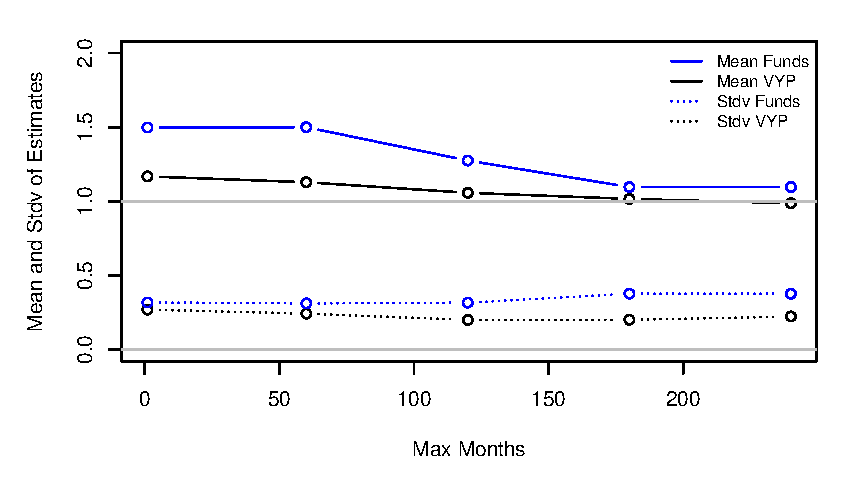
\includegraphics{eps/Simulationfundsvsvyps}
	\caption{Simulation results comparing individual funds vs. vintage year portfolios (VYPs) with true $\beta=1$ and simple linear SDF.}
	\label{fig:simulation_funds_vs_vyps}
\end{figure}


\paragraph{SDF model $\Psi$:}
In our base case with vintage year portfolios, the exponential affine SDF shows a mean and standard deviation of 1.011 (0.175) compared to the 1.016 (0.2) achieved by the simple linear SDF.
Generally, the exponential affine SDF model and the simple linear SDF model exhibit similar bias and variance when comparing panels A and B in table \ref{tab:simulation_study}.
Figure \ref{fig:simulation_expaff_vs_simlin} visualizes the true $\beta=1$ case which shows that the estimation results are not overly sensitive to the choice of the SDF model.

Moreover, the perceived superiority of exponential affine SDFs is probably rather theoretical than practical as other proponents also emphasize their universality mainly from a mathematical perspective without providing supportive empirical or simulation results \citep{GM07,BMP08}.

\begin{figure}
	\centering
	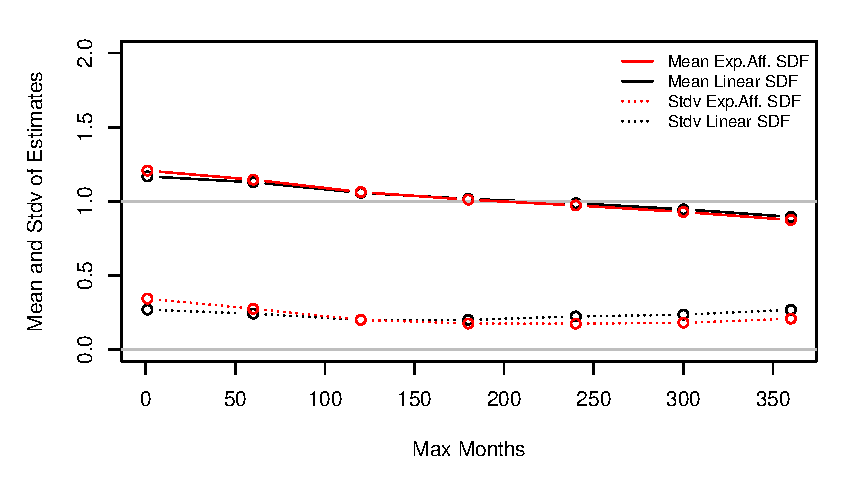
\includegraphics{eps/Simulationexpaffvssimlin}
	\caption{Simulation results comparing exponentially affine and simple linear SDF with true $\beta=1$ and vintage year portfolios.}
	\label{fig:simulation_expaff_vs_simlin}
\end{figure}


\paragraph{Varying vintages $V$ and portfolio sizes $n/V$:}
To test the effect of varying data sizes available for MKT factor estimation, we in/decrease the (i) number of vintage years and (ii) the number of funds per vintage year (cf. table \ref{tab:simulation_study_size}).
Here we use vintage year portfolios and the simple linear SDF.
For our simple data generating process, increasing the number of deals/funds per vintage year portfolio appears to decrease the estimator's variance more effectively than adding more vintage years.
However, the bias is almost the same for all tested specifications.
Generally, we seem to need many new data points to ensure a reasonable variance of our estimator.

\begin{table}[ht]
	\centering
	\begin{tabular}{rrrrrrr}
		& Base & Big $n/V$ & Big $V$ & Big $V$ & Small $V$ & Small $V$ \\ 
		\hline
		\hline
		Start vintage & 1986 & 1986 & 1967 & 1967 & 1986 & 1996 \\ 
		End vintage & 2005 & 2005 & 2005 & 2005 & 1995 & 2005 \\ 
		\#Funds per vintage & 20 & 40 & 10 & 20 & 20 & 20 \\ 
		\hline
		Mean $\beta_{\mathrm{MKT}}$ & 1.011 & 1.020 & 0.993 & 1.015 & 1.027 & 0.934 \\ 
		Stdv $\beta_{\mathrm{MKT}}$ & 0.187 & 0.133 & 0.263 & 0.227 & 0.232 & 0.418 \\ 
		\hline
		\hline
	\end{tabular}
	\caption{Simulation study for varying  number of vintages and number of funds per vintage. 
		   We use vintage year portfolios, the simple linear SDF with true $\beta_{\mathrm{MKT}}=1$, maximum month 180, and 500 simulation iterations.} 
	\label{tab:simulation_study_size}
\end{table}

\paragraph{Size of set $\mathcal{T}$:}
The results in table \ref{tab:simulation_study} indicate that we can control the bias by an appropriate choice of the set $\mathcal{T}$.
The bias almost vanishes when we average over all present value dates in the maximal fund lifetime of 180 months. 
For smaller or larger sets for $\mathcal{T}$, we find increasing small-sample bias\footnote{Recall that using the minimal set for $\mathcal{T}$, i.e., discounting all cash flows just to the fund inception date, corresponds exactly to the \cite{DLP12} approach. Thus, the original \cite{DLP12} methodology achieves a suboptimal small-sample bias since it does not average pricing errors over multiple present value dates.}.

The same finding also holds when we limit the maximal fund lifetime to ten years by reducing the maximum deal holding period from ten to five years. 
Here, under correct model specification with $\beta_{\mathrm{MKT}}=1$ , the smallest bias is obtained for maximum month 120:
for max. month 60 we get 1.028 (0.116), for max. month 120 we get 1.005 (0.116), and for max. month 180 we get 0.969 (0.13).

In table \ref{tab:simulation_study} for both true and false model specifications, the $\alpha$ standard deviation is very high compared to its mean value.
This may indicate it is rather delicate to empirically determine private equity's historical outperformance by our semiparametric estimator. \newline

To conclude, our simulations study rationalizes two key practices from the \cite{DLP12} paper: (i) vintage year portfolio formation helps to improve estimator precision and (ii) increasing the number of funds per vintage seems to be more effective in controlling estimator variance that increasing the number of vintages\footnote{Finding (ii) may explain the choice of \cite{DLP12} to employ an asymptotic law that lets the number of deals/funds per vintage tend to infinity.}.
However, our examples with correct specification cannot support the assumption of \cite{KN16} that (iii) the exponential affine SDF is (clearly) superior to the simple liner SDF in a multi-period framework; actually, their bias and variances are quite equal.
Moreover, our simulation study suggests that (iv) averaging pricing errors over multiple dates strikingly reduces the bias inherent to the original procedure of \cite{DLP12} that just discounts all cash flows to the fund inception date.
Actually, choosing the set $\mathcal{T}$ according to the fund lifetime seems to decrease the bias (and to a lesser extend also the variance) more effectively than all other measures combined.



\subsection{Empirical results}

Following the conclusions from the previous subsection, we use vintage year portfolios to estimate simple linear SDF models with maximum month 180.
Asymptotic inference results for the full dataset are exhibited in table \ref{tab:ai_180_FW_VYP_SL} for fund-size weighting and in table \ref{tab:ai_180_EW_VYP_SL} for equal weighting.
The results for $hv$-block cross-validation are displayed in table \ref{tab:cv_180_FW_VYP_SL} for fund-size weighting and in table \ref{tab:cv_180_EW_VYP_SL} for equal weighting.
We generally analyze the results in a two-step procedure: For a given model specification, we use the cross-validation error (i.e., the average out-of-sample error) to select the best model for each fund type, but analyze the corresponding coefficient estimates from the asymptotic inference tables (estimated on the entire data set).
Therefore, for each fund type the SDF models in the asymptotic inference tables \ref{tab:ai_180_FW_VYP_SL} and \ref{tab:ai_180_EW_VYP_SL} are sorted by the corresponding cross-validation error.
Throughout this subsection, we define the statistical significance of coefficient estimates in terms of a $t$-ratio $\hat{\theta}[SE(\hat{\theta})]^{-1}$ greater than 1.96.

% latex table generated in R 3.4.2 by xtable 1.8-4 package
% Mon Jun  8 20:27:19 2020
\begin{table}[ht]
	\centering
	\begin{tabular}{llrrrrrr}
		& & \multicolumn{3}{l}{MKT Factor} & \multicolumn{3}{l}{Second Factor} \\ 
		Weighting & Inference & Coef & SE & SE.indep & Coef & SE & SE.indep \\ 
		\hline
		\hline
		fund-size & asymptotic & 0.75 & 27.06 & 19.73 & 0.80 & 28.95 & 20.94 \\ 
		fund-size & cross-validation & 0.85 & 0.38 & - & 0.59 & 0.51 & - \\ 
		\hline
		equal & asymptotic & 0.76 & 26.75 & 16.16 & 0.76 & 11.25 & 6.69 \\ 
		equal & cross-validation & 0.84 & 0.34 & - & 0.62 & 0.50 & - \\ 
		\hline
		\hline
	\end{tabular}
	\caption{
		Top-level overview over tables \ref{tab:ai_180_FW_VYP_SL} to \ref{tab:cv_180_EW_VYP_SL}: 
		Averages of absolute values of coefficient estimates and standard errors.
	} 
	\label{tab:ai_sum_abs}
\end{table}

Table \ref{tab:ai_sum_abs} helps to get a rough overview of tables \ref{tab:ai_180_FW_VYP_SL} to \ref{tab:cv_180_EW_VYP_SL} as it summarizes their absolute column means.
Conspicuously, asymptotic standard errors (SEs) seem enormously high and, moreover, contain colossal outliers.
The standard errors implied by $hv-$block cross-validation are considerably smaller than the asymptotic SEs and seem to lie within a plausible range.
When just looking at asymptotic standard errors of the second factors, fund-size weighting exhibits substantially larger SEs than fund equal-weighting.
Assuming independence between funds from different vintages decreases asymptotic SEs by approximately 30-40\% compared to a realistic kernel bandwidth of $D=12$.
But even these independent SEs rarely imply statistical significance coefficient estimates with $t$-ratios bigger than 1.96.
In table \ref{tab:ai_180_FW_VYP_SL} with fund-size weighting, just one out of 36 models exhibit asymptotically significant MKT and second-factor estimates.
In the case of equal-weighting, table \ref{tab:ai_180_EW_VYP_SL} also shows just one asymptotically significant model out of 36.

In summary, the results reveal weak two-factor models with MKT plus a second $q$-investment factor. 
Likewise, the simulation results from the previous subsection indicate a rather high variance associated with our semiparametric estimator (given the amount of data typically available).
Thus, we recommend focusing on single MKT factor models even when their asymptotic t-ratios are below 1.96.
At least the $hv$-block cross-validation standard deviations imply significant one-factor MKT models for fund types PE, VC, PD, INF.
In contrast, RE is just significant for equal-weighting, and NR is insignificant for both weighting schemes.

\paragraph{Focus on PE and VC estimates}

Here, we briefly summarize the one-factor MKT and the two-factor Alpha model estimates for fund types PE (i.e., mainly Buyout and Growth) and VC.
For PE, all one-factor MKT model $\beta_{\mathrm{MKT}}$ estimates fall in the range from 1.13 to 1.28. 
If we add an $\alpha$ term, all $\beta_{\mathrm{MKT}}$ estimates decrease to the range 0.61 to 0.77 with annualized $\alpha$ coefficients of approximately positive 4-5\% per year.
For VC, the one-factor MKT model $\beta_{\mathrm{MKT}}$ estimates are in the range from 0.80 to 1.14.
If we add an $\alpha$ term, all $\beta_{\mathrm{MKT}}$ estimates strongly increase to the range 1.81 to 2.06 with annualized $\alpha$ coefficients of approximately negative 6-7\% per year.
These results at least weakly indicate - given their insignificant asymptotic standard errors - that PE funds outperform public markets with a market beta coefficient of less than one, which suggests low market risk.
On the other hand, VC underperforms public markets with market beta coefficients of roughly two, which implies high market risk.
So, even \cite{DLP12} use the problematic Thomson Venture Economics (TVE) dataset for their empirical analysis\footnote{\cite{HJK14} discuss the potential downward bias of the TVE dataset.}, we obtain similar qualitative results using Preqin data: (i) the market beta of VC seems to be higher than that of PE and (ii) VC, in contrast to PE, appears to exhibit a negative abnormal performance $\alpha$.

As a robustness check, we reestimate all SDF models on a dataset that just contains funds from vintages older or equal than 2011.
Interestingly, the PE and VC results regarding $\beta_{\mathrm{MKT}}$ and $\alpha$ can be qualitatively and also quantitatively confirmed on this 'mostly-liquidated' dataset\footnote{All R code and data is available in an online repository. %\url{https://github.com/quant-unit/Fundwise_SDF/tree/master/r_project}
}.




\section{Conclusion}
\label{sec:conclusion}

Theoretically, our Least-Mean-Distance estimator can be easily generalized to estimate SDF models for all kinds of non-traded cash flows.
Practically, semiparametric estimators commonly exhibit problematic small sample behavior.
Given the amount of currently available private equity fund data, our estimator's variance seems quite large, even for simple SDF model specifications.
Specifically, our Monte Carlo simulation results prompt us to conclude that the closely related \cite{DLP12} estimator may exhibit more bias and variance than originally assumed in their paper.
Especially, the variance of $\alpha$ estimates seems to be too high to allow reliable abnormal performance conclusions.
Fortunately, we show that at least the bias can be easily reduced by averaging pricing errors over all dates within the fund lifetime.

In the data-sparse private equity domain with only 20-40 cross-sectional units (i.e., vintage year portfolios) currently available for estimation, asymptotic inference seems not to be overly useful.
Thus, we strongly advise to always challenge asymptotic inference results by resampling or cross-validation techniques that are adapted to the dependence structure of overlapping fund cash flows.
However, even their conclusions should be double-checked, to avoid unreasonable instances, e.g., when $hv$-block cross-validation chooses dubious models with negative MKT factor estimates.
Since, in our empirical analyses, basically all two-factor models' asymptotic standard errors appear statistically insignificant, we conjecture that naive versions of our SDF estimator shall be exclusively used for a single-MKT-factor model until considerably more vintage year information for private equity funds is available.

If someone wants to estimate more complex SDF models that incorporate additional factors, more structure is needed.
This can be parametric assumptions for the data generating process \citep{ACGP18} or to extract additional information from intermediate net asset values \citep{GSW19,BGG20}.
A first 'modern' approach to the same problem is applying machine learning techniques that regularize/shrink all coefficients other than the MKT factor.
Secondly, given the high estimator variance revealed in the simulation study, statistical learning methods that create a strong learner by combining multiple weak learners seem also worth considering (boosting, bagging, model averaging).
%However, as our least-mean-distance estimator can be perceived as a simple special case of a GMM estimator (with ex-ante fixed identity weighting matrix), we cannot recommend GMM application in our context since even the simpler version delivers merely weak results.


%% References
\bibliographystyle{apalike}
\bibliography{xfundwise_sdf}



% Appendix


\newpage


\begin{table}[ht]
	\centering
	\begin{tabular}{lrrrrrr}
		\multicolumn{7}{c}{Panel A: simple linear SDF} \\
		\hline
		Model==DGP & True & \multicolumn{2}{c}{False} & False & \multicolumn{2}{c}{True} \\
		MaxMonth & $\beta=1$ & $\alpha=0$ & $\beta=1$ & $\beta=2.5$ & $\alpha=-0.25$ & $\beta=2.5$ \\ 
		\hline
		\hline
		1 - mean & 1.168 & 1625\% & 0.003 & 2.023 & 5879\% & -16.711 \\ 
		1 - stdv & 0.269 & 2792\% & 9.968 & 0.342 & 866\% & 13.347 \\ 
		\hline
		60 - mean & 1.129 & 0.138\% & 0.933 & 2.103 & -0.086\% & 2.285 \\ 
		60 - stdv & 0.242 & 0.245\% & 0.363 & 0.302 & 0.253\% & 0.406 \\ 
		\hline
		120 - mean & 1.058 & 0.112\% & 0.906 & 2.063 & -0.085\% & 2.239 \\ 
		120 - stdv & 0.200 & 0.214\% & 0.313 & 0.253 & 0.239\% & 0.385 \\ 
		\hline
		180 - mean & 1.016 & 0.041\% & 0.965 & 2.052 & -0.161\% & 2.370 \\ 
		180 - stdv & 0.200 & 0.172\% & 0.334 & 0.277 & 0.173\% & 0.403 \\ 
		\hline
		240 - mean & 0.987 & -0.053\% & 1.077 & 2.072 & -0.277\% & 2.589 \\ 
		240 - stdv & 0.223 & 0.162\% & 0.361 & 0.326 & 0.118\% & 0.375 \\
		\hline 
		300 - mean & 0.946 & -0.149\% & 1.175 & 2.080 & -0.357\% & 2.714 \\ 
		300 - stdv & 0.235 & 0.174\% & 0.377 & 0.398 & 0.114\% & 0.366 \\ 
		\hline
		360 - mean & 0.895 & -0.245\% & 1.269 & 2.048 & -0.461\% & 2.859 \\ 
		360 - stdv & 0.268 & 0.201\% & 0.399 & 0.551 & 0.140\% & 0.386 \\ 
		\hline
		\hline
		\multicolumn{7}{l}{} \\
		\multicolumn{7}{c}{Panel B: exponential affine SDF} \\
		\hline
		Model==DGP & True & \multicolumn{2}{c}{False} & False & \multicolumn{2}{c}{True} \\
		MaxMonth & $\beta=1$ & $\alpha=0$ & $\beta=1$ & $\beta=2.5$ & $\alpha=-0.25$ & $\beta=2.5$ \\ 
		\hline
		\hline
		1 - mean & 1.207 & 203\% & 1.276 & 2.256 & 692\% & 1.704 \\ 
		1 - stdv & 0.344 & 314\% & 0.710 & 0.290 & 13\% & 1.666 \\ 
		\hline
		60 - mean & 1.146 & 0.126\% & 0.941 & 2.264 & -0.018\% & 2.277 \\ 
		60 - stdv & 0.275 & 0.264\% & 0.386 & 0.256 & 0.370\% & 0.473 \\ 
		\hline
		120 - mean & 1.062 & 0.107\% & 0.908 & 2.221 & 0.009\% & 2.205 \\ 
		120 - stdv & 0.200 & 0.237\% & 0.333 & 0.187 & 0.357\% & 0.448 \\ 
		\hline
		180 - mean & 1.011 & 0.027\% & 0.971 & 2.182 & -0.136\% & 2.358 \\ 
		180 - stdv & 0.175 & 0.211\% & 0.366 & 0.168 & 0.344\% & 0.505 \\ 
		\hline
		240 - mean & 0.972 & -0.088\% & 1.095 & 2.144 & -0.441\% & 2.723 \\ 
		240 - stdv & 0.174 & 0.224\% & 0.406 & 0.178 & 0.317\% & 0.503 \\ 
		\hline
		300 - mean & 0.928 & -0.202\% & 1.203 & 2.083 & -0.717\% & 2.985 \\ 
		300 - stdv & 0.181 & 0.253\% & 0.426 & 0.254 & 0.340\% & 0.513 \\ 
		\hline
		360 - mean & 0.874 & -0.319\% & 1.304 & 1.685 & -1.095\% & 3.272 \\ 
		360 - stdv & 0.208 & 0.291\% & 0.447 & 0.772 & 0.374\% & 0.586 \\ 
		\hline
		\hline
	\end{tabular}
	\caption{
		Simulation study to compare the simple linear with the exponential affine SDF and to determine the optimal size of the set $\mathcal{T}$.
		Here, we always use vintage year portfolios and 1000 simulation iterations.
		For better readability, $\beta_{\mathrm{MKT}}=\beta$.
		For the unity and high beta model, we test true and false model specifications (with and without the $\alpha$ term).
	} 
	\label{tab:simulation_study}
\end{table}




% latex table generated in R 3.4.2 by xtable 1.8-4 package
% Mon Jun  8 17:19:54 2020
\begin{table}[ht]
	\centering
	\begin{tabular}{lrrrlrrr}
		 & \multicolumn{3}{l}{MKT Factor} & & \multicolumn{3}{l}{Second Factor} \\ 
		Type & Estim. & SE & SE.indep & Factor & Estim. & SE & SE.indep \\ 
		\hline
		\hline
PE & 0.709 & 2.470 & 1.153 & EG & 0.807 & 4.693 & 1.960 \\ 
PE & 0.770 & 7.976 & 3.348 & ROE & 1.540 & 5.140 & 3.499 \\ 
PE & 1.126 & 1.003 & 0.868 & MKT & 1.126 & 1.003 & 0.868 \\ 
PE & 0.644 & 1.234 & 0.585 & Alpha & 0.003 & 0.036 & 0.013 \\ 
PE & 1.121 & 1.023 & 0.897 & ME & 0.074 & 2.021 & 0.915 \\ 
PE & 1.158 & 1.125 & 1.068 & IA & -0.338 & 2.499 & 1.259 \\
\hline 
VC & 1.053 & 4.150 & 2.733 & IA & -1.959 & 2.100 & 1.767 \\ 
VC & 1.114 & 3.861 & 2.894 & ME & -1.383 & 5.102 & 2.211 \\ 
VC & 1.806 & 11.391 & 4.279 & Alpha & -0.006 & 0.124 & 0.046 \\ 
VC & 0.801 & 704.455 & 561.598 & MKT & 0.801 & 704.455 & 561.598 \\ 
VC & 1.429 & 8.073 & 3.219 & ROE & -1.306 & 18.055 & 6.919 \\ 
VC & 1.507 & 17.322 & 6.966 & EG & -0.904 & 15.344 & 5.737 \\ 
\hline
PD & 0.885 & 1.040 & 1.242 & MKT & 0.885 & 1.040 & 1.242 \\ 
PD & 0.660 & 0.095 & 0.039 & Alpha & 0.002 & 0.001 & 0.000 \\ 
PD & 0.826 & 1.707 & 1.443 & EG & 0.143 & 20.341 & 7.506 \\ 
PD & 0.849 & 2.921 & 2.146 & ME & 0.301 & 2.739 & 1.518 \\ 
PD & 0.887 & 1.378 & 1.244 & ROE & -0.023 & 6.925 & 2.553 \\ 
PD & 0.863 & 2.942 & 2.224 & IA & 0.247 & 5.306 & 3.607 \\ 
\hline
RE & 0.578 & 1.827 & 1.196 & MKT & 0.578 & 1.827 & 1.196 \\ 
RE & 1.303 & 5.463 & 2.259 & Alpha & -0.006 & 0.088 & 0.034 \\ 
RE & 0.200 & 2.598 & 1.356 & ROE & 3.118 & 2.579 & 6.629 \\ 
RE & 0.202 & 3.297 & 1.965 & EG & 0.844 & 2.478 & 1.828 \\ 
RE & 0.756 & 3.043 & 2.192 & IA & -1.938 & 1.879 & 0.783 \\ 
RE & 0.887 & 1.167 & 0.858 & ME & -2.059 & 1.300 & 0.563 \\ 
\hline
NR & -0.215 & 2.367 & 1.976 & EG & 0.909 & 14.505 & 7.475 \\ 
NR & 0.191 & 3.136 & 4.242 & MKT & 0.191 & 3.136 & 4.242 \\ 
NR & -0.674 & 58.003 & 24.234 & Alpha & 0.008 & 0.230 & 0.098 \\ 
NR & -0.020 & 0.954 & 2.210 & ROE & 1.128 & 4.830 & 5.066 \\ 
NR & 0.143 & 3.236 & 4.116 & IA & -0.768 & 1.808 & 2.154 \\ 
NR & 0.212 & 4.209 & 5.450 & ME & -0.575 & 1.603 & 1.252 \\ 
\hline
INF & 0.824 & 3.201 & 2.815 & MKT & 0.824 & 3.201 & 2.815 \\ 
INF & 0.190 & 7.133 & 3.288 & Alpha & 0.005 & 0.030 & 0.025 \\ 
INF & 0.317 & 23.904 & 10.658 & EG & 0.848 & 45.836 & 20.176 \\ 
INF & 0.470 & 9.316 & 4.237 & ROE & 1.245 & 5.531 & 6.134 \\ 
INF & 0.778 & 5.951 & 5.424 & ME & -0.811 & 3.712 & 4.349 \\ 
INF & 0.661 & 61.329 & 33.819 & IA & -1.108 & 150.713 & 85.733 \\ 
		\hline
		\hline
	\end{tabular}
	\caption{Asymptotic inference with fund-size-weighting, max month 180, and $D=12$.} 
	\label{tab:ai_180_FW_VYP_SL}
\end{table}


\begin{table}[ht]
	\centering
	\begin{tabular}{lrrlrrr}
		 & \multicolumn{2}{l}{MKT Factor} & & \multicolumn{2}{l}{Second Factor} & \\ 
		Type & Mean & SD & Factor & Mean & SD & CV-error \\ 
		\hline
		\hline
PE & 0.867 & 0.276 & EG & 0.720 & 0.137 & 112808.000 \\ 
PE & 0.927 & 0.305 & ROE & 1.375 & 0.420 & 126801.000 \\ 
PE & 1.276 & 0.296 & MKT & 1.276 & 0.296 & 151964.000 \\ 
PE & 0.772 & 0.238 & Alpha & 0.004 & 0.002 & 154805.000 \\ 
PE & 1.317 & 0.396 & ME & 0.236 & 0.664 & 209319.000 \\ 
PE & 1.311 & 0.370 & IA & 0.014 & 0.703 & 210650.000 \\ 
\hline
VC & 1.045 & 0.126 & IA & -1.890 & 0.238 & 11858.000 \\ 
VC & 1.172 & 0.126 & ME & -1.448 & 0.263 & 13301.000 \\ 
VC & 1.930 & 0.356 & Alpha & -0.005 & 0.001 & 17723.000 \\ 
VC & 0.804 & 0.363 & MKT & 0.804 & 0.363 & 21852.000 \\ 
VC & 1.527 & 0.517 & ROE & -0.972 & 0.679 & 26680.000 \\ 
VC & 1.646 & 0.678 & EG & -0.644 & 0.556 & 32730.000 \\ 
\hline
PD & 0.887 & 0.039 & MKT & 0.887 & 0.039 & 7368.000 \\ 
PD & 0.567 & 0.202 & Alpha & 0.003 & 0.001 & 7917.000 \\ 
PD & 0.763 & 0.113 & EG & 0.229 & 0.141 & 8758.000 \\ 
PD & 0.862 & 0.103 & ME & 0.342 & 0.256 & 9834.000 \\ 
PD & 0.812 & 0.153 & ROE & 0.258 & 0.394 & 11522.000 \\ 
PD & 0.914 & 0.211 & IA & 0.472 & 0.424 & 18096.000 \\
\hline 
RE & 0.722 & 0.392 & MKT & 0.722 & 0.392 & 50900.000 \\ 
RE & 1.288 & 0.345 & Alpha & -0.004 & 0.005 & 51437.000 \\ 
RE & 0.389 & 0.446 & ROE & 2.333 & 1.507 & 54689.000 \\ 
RE & 0.465 & 0.470 & EG & 0.448 & 0.629 & 59316.000 \\ 
RE & 0.847 & 0.411 & IA & -1.262 & 1.160 & 65835.000 \\ 
RE & 0.983 & 0.350 & ME & -1.467 & 1.298 & 66827.000 \\ 
\hline
NR & -0.047 & 0.421 & EG & 0.657 & 0.557 & 10559.000 \\ 
NR & 0.318 & 0.321 & MKT & 0.318 & 0.321 & 11480.000 \\ 
NR & -0.335 & 0.763 & Alpha & 0.006 & 0.005 & 11854.000 \\ 
NR & 0.136 & 0.466 & ROE & 0.844 & 1.062 & 13296.000 \\ 
NR & 0.270 & 0.508 & IA & -0.288 & 1.124 & 14479.000 \\ 
NR & 0.416 & 0.587 & ME & 0.032 & 1.079 & 15789.000 \\ 
\hline
INF & 0.862 & 0.320 & MKT & 0.862 & 0.320 & 14551.000 \\ 
INF & 0.639 & 0.753 & Alpha & 0.002 & 0.004 & 15069.000 \\ 
INF & 0.766 & 0.626 & EG & 0.258 & 0.495 & 16004.000 \\ 
INF & 0.837 & 0.504 & ROE & 0.090 & 0.939 & 18472.000 \\ 
INF & 0.868 & 0.412 & ME & 0.078 & 0.643 & 18514.000 \\ 
INF & 0.892 & 0.561 & IA & 0.081 & 1.073 & 23162.000 \\ 
		\hline
		\hline
	\end{tabular}
	\caption{$hv$-block cross-validation with fund-size-weighting and max month 180.} 
	\label{tab:cv_180_FW_VYP_SL}
\end{table}


% latex table generated in R 3.4.2 by xtable 1.8-4 package
% Mon Jun  8 17:44:27 2020
\begin{table}[ht]
	\centering
	\begin{tabular}{lrrrlrrr}
		 & \multicolumn{3}{l}{MKT Factor} & & \multicolumn{3}{l}{Second Factor} \\ 
		Type & Estim. & SE & SE.indep & Factor & Estim. & SE & SE.indep \\ 
		\hline
		\hline
PE & 0.775 & 0.638 & 0.550 & EG & 0.667 & 5.558 & 2.125 \\ 
PE & 0.610 & 1.064 & 0.387 & Alpha & 0.004 & 0.006 & 0.002 \\ 
PE & 0.826 & 20.352 & 8.308 & ROE & 1.087 & 33.514 & 12.143 \\ 
PE & 1.134 & 1.050 & 0.694 & MKT & 1.134 & 1.050 & 0.694 \\ 
PE & 1.146 & 1.001 & 0.638 & IA & -0.386 & 1.909 & 0.813 \\ 
PE & 1.134 & 1.048 & 0.702 & ME & -0.014 & 1.797 & 0.736 \\ 
\hline
VC & 1.181 & 24.418 & 16.693 & ME & -1.277 & 4.928 & 4.352 \\ 
VC & 1.137 & 7.259 & 6.057 & IA & -1.553 & 3.716 & 2.139 \\ 
VC & 1.956 & 4.189 & 1.520 & Alpha & -0.006 & 0.335 & 0.117 \\ 
VC & 1.034 & 2.205 & 1.758 & MKT & 1.034 & 2.205 & 1.758 \\ 
VC & 1.488 & 1.801 & 0.941 & ROE & -1.148 & 4.060 & 1.424 \\ 
VC & 1.535 & 2.821 & 1.336 & EG & -0.754 & 3.626 & 1.260 \\ 
\hline
PD & 0.844 & 1.245 & 0.856 & MKT & 0.844 & 1.245 & 0.856 \\ 
PD & 0.502 & 0.044 & 0.015 & Alpha & 0.003 & 0.000 & 0.000 \\ 
PD & 0.791 & 2.478 & 1.557 & ROE & 0.222 & 5.024 & 1.966 \\ 
PD & 0.736 & 2.230 & 1.303 & EG & 0.213 & 6.296 & 2.374 \\ 
PD & 0.844 & 1.150 & 0.837 & IA & 0.076 & 2.543 & 1.416 \\ 
PD & 0.833 & 1.978 & 1.362 & ME & 0.323 & 1.845 & 0.986 \\ 
\hline
RE & 0.743 & 3.471 & 2.075 & MKT & 0.743 & 3.471 & 2.075 \\ 
RE & 1.265 & 7.581 & 3.331 & Alpha & -0.004 & 0.046 & 0.017 \\ 
RE & 0.145 & 3.486 & 1.614 & ROE & 3.202 & 17.447 & 7.413 \\ 
RE & 0.400 & 50.493 & 31.818 & EG & 0.700 & 48.813 & 29.195 \\ 
RE & 0.884 & 4.928 & 2.813 & ME & -1.782 & 1.474 & 0.605 \\ 
RE & 0.795 & 18.146 & 10.282 & IA & -1.712 & 13.199 & 7.657 \\ 
\hline
NR & -0.056 & 3.693 & 1.897 & ROE & 1.934 & 3.154 & 2.287 \\ 
NR & 0.000 & 4.771 & 2.368 & EG & 0.814 & 1.368 & 1.753 \\ 
NR & 0.425 & 3.370 & 5.178 & MKT & 0.425 & 3.370 & 5.178 \\ 
NR & -0.272 & 39.463 & 16.698 & Alpha & 0.006 & 0.202 & 0.081 \\ 
NR & 0.394 & 0.871 & 1.401 & IA & -0.319 & 1.734 & 1.169 \\ 
NR & 0.453 & 15.719 & 24.377 & ME & 0.432 & 5.574 & 8.016 \\ 
\hline
INF & 0.098 & 0.055 & 0.025 & Alpha & 0.006 & 0.001 & 0.000 \\ 
INF & 0.280 & 20.158 & 8.983 & EG & 0.893 & 21.368 & 9.700 \\ 
INF & 0.775 & 19.273 & 22.509 & MKT & 0.775 & 19.273 & 22.509 \\ 
INF & 0.469 & 26.226 & 12.751 & ROE & 1.030 & 30.728 & 16.129 \\ 
INF & 0.758 & 33.453 & 36.239 & ME & -0.804 & 16.214 & 16.161 \\ 
INF & 0.664 & 630.801 & 351.730 & IA & -0.929 & 137.937 & 75.628 \\ 
		\hline
		\hline
	\end{tabular}
	\caption{Asymptotic inference with equal-weighting, max month 180, and $D=12$.} 
	\label{tab:ai_180_EW_VYP_SL}
\end{table}

% latex table generated in R 3.4.2 by xtable 1.8-4 package
% Mon Jun  8 17:44:27 2020
\begin{table}[ht]
	\centering
	\begin{tabular}{lrrlrrr}
		 & \multicolumn{2}{l}{MKT Factor} & & \multicolumn{2}{l}{Second Factor} & \\ 
		Type & Mean & SD & Factor & Mean & SD & CV-error \\ 
		\hline
		\hline
PE & 0.886 & 0.262 & EG & 0.614 & 0.217 & 101444.000 \\ 
PE & 0.719 & 0.205 & Alpha & 0.004 & 0.001 & 105842.000 \\ 
PE & 0.948 & 0.267 & ROE & 0.975 & 0.407 & 110926.000 \\ 
PE & 1.250 & 0.262 & MKT & 1.250 & 0.262 & 127589.000 \\ 
PE & 1.247 & 0.274 & IA & -0.183 & 0.598 & 157037.000 \\ 
PE & 1.281 & 0.323 & ME & 0.048 & 0.644 & 169552.000 \\ 
\hline
VC & 1.250 & 0.153 & ME & -1.292 & 0.234 & 16305.000 \\ 
VC & 1.183 & 0.169 & IA & -1.507 & 0.327 & 16449.000 \\ 
VC & 2.052 & 0.257 & Alpha & -0.006 & 0.001 & 18666.000 \\ 
VC & 1.138 & 0.341 & MKT & 1.138 & 0.341 & 25321.000 \\ 
VC & 1.610 & 0.431 & ROE & -0.946 & 0.426 & 26618.000 \\ 
VC & 1.688 & 0.505 & EG & -0.616 & 0.331 & 30392.000 \\ 
\hline
PD & 0.838 & 0.029 & MKT & 0.838 & 0.029 & 11290.000 \\ 
PD & 0.458 & 0.151 & Alpha & 0.003 & 0.001 & 11568.000 \\ 
PD & 0.770 & 0.058 & ROE & 0.232 & 0.111 & 11572.000 \\ 
PD & 0.707 & 0.086 & EG & 0.224 & 0.091 & 12194.000 \\ 
PD & 0.825 & 0.083 & IA & 0.158 & 0.305 & 15071.000 \\ 
PD & 0.837 & 0.098 & ME & 0.358 & 0.328 & 15441.000 \\ 
\hline
RE & 0.803 & 0.336 & MKT & 0.803 & 0.336 & 43486.000 \\ 
RE & 1.191 & 0.363 & Alpha & -0.003 & 0.004 & 45310.000 \\ 
RE & 0.341 & 0.402 & ROE & 2.275 & 1.558 & 52822.000 \\ 
RE & 0.559 & 0.379 & EG & 0.397 & 0.503 & 52867.000 \\ 
RE & 0.929 & 0.339 & ME & -1.287 & 1.174 & 57341.000 \\ 
RE & 0.852 & 0.372 & IA & -1.129 & 1.025 & 57662.000 \\ 
\hline
NR & -0.009 & 0.203 & ROE & 1.880 & 0.562 & 15631.000 \\ 
NR & 0.200 & 0.510 & EG & 0.681 & 0.372 & 18981.000 \\ 
NR & 0.572 & 0.400 & MKT & 0.572 & 0.400 & 20006.000 \\ 
NR & -0.065 & 0.729 & Alpha & 0.006 & 0.004 & 20880.000 \\ 
NR & 0.596 & 0.567 & IA & -0.060 & 0.869 & 24766.000 \\ 
NR & 0.769 & 0.771 & ME & 0.666 & 1.062 & 27238.000 \\ 
\hline
INF & 0.124 & 0.608 & Alpha & 0.007 & 0.006 & 14995.000 \\ 
INF & 0.613 & 0.393 & EG & 0.402 & 0.496 & 15758.000 \\ 
INF & 0.862 & 0.281 & MKT & 0.862 & 0.281 & 15820.000 \\ 
INF & 0.627 & 0.360 & ROE & 0.577 & 1.374 & 18297.000 \\ 
INF & 0.810 & 0.315 & ME & -0.129 & 1.109 & 19641.000 \\ 
INF & 0.797 & 0.842 & IA & 0.051 & 2.180 & 33661.000 \\ 
		\hline
		\hline
	\end{tabular}
	\caption{$hv$-block cross-validation with equal-weighting and max month 180.} 
	\label{tab:cv_180_EW_VYP_SL}
\end{table}





\end{document}
